\documentclass[a4paper, 10pt]{article}
\usepackage[latin1]{inputenc}          % Accept european-encoded (latin1) characters.
\usepackage{a4wide}                    % Wide paper
\usepackage[parfill]{parskip}          % skip a line instead of indenting new paragraphs
\usepackage{graphicx}                  % For eps figures
\usepackage{epsfig}                    % Alternative package
\usepackage{hyperref}
\hypersetup
{
  colorlinks=false,
  pdfborder={0,0,0},
}
 
\usepackage{fancyhdr}
\fancyhead[L]{\class \;- \assignment }
\fancyhead[R]{\author }
\renewcommand{\footrulewidth}{0.5pt} % Insert a line above the footer
\pagestyle{fancy}
\usepackage[hang,small,bf]{caption}
\usepackage{palatino}
\usepackage{amsmath}
\usepackage{amssymb}
\usepackage{enumerate}
 
% convenience commands
\renewcommand{\author}{Daniel Standage}
\newcommand{\class}{BCB 568}
\newcommand{\instructor}{Brendel/Dorman}
\newcommand{\assignment}{HW 3}
\newcommand{\duedate}{Feb 3, 2011}
 
\newcounter{prob_num}
\setcounter{prob_num}{1}
% usage: \problem
\newcommand{\problem}{\vspace{20pt}\arabic{prob_num}.\stepcounter{prob_num}\par}
% usage: \head{name}{class}{assignment}
\newcommand{\head}{\begin{center}\begin{tabular*}{\linewidth}{l@{\extracolsep{\fill}}r} & \class \;- \assignment \\ & \duedate \end{tabular*}\end{center} \hfill }
% usage: \eqn{equation}{label}
\newcommand{\eqn}[2]{\begin{equation}#1\label{#2}\end{equation}}
 
\begin{document}

%%%%%%%%%%%%%%%%%%%%%%%%%%%%%%%%%%%%%%%%%%%%%%%%%%
\problem

Let $\mu$ be the waiting time until observing $ATG$ in the sequence and $\mu_{S'}$ be the waiting time until observing $ATG$ from the pattern $S'$. We can use first step analysis and the given base probabilities to establish the following system of equations.
\begin{eqnarray}
  \mu           &=& 1 + P_A \mu_A + (1 - P_A)\mu_{\bar{A}} \nonumber \\
  \mu_{\bar{A}} &=& 1 + P_A \mu_A + (1 - P_A)\mu_{\bar{A}} \nonumber \\
  \mu_A         &=& 1 + P_A \mu_A + (P_C + P_G)\mu_{\bar{A}} + P_T\mu_{AT} \nonumber \\
  \mu_{AT}      &=& 1 + P_A \mu_A + (P_C + P_T)\mu_{\bar{A}} + P_G\mu_{ATG} \nonumber \\
  \mu_{ATG}     &=& 0 \nonumber
\end{eqnarray}

Solving this system, we get \[ \mu = \frac{1}{P_A P_T P_G} = \frac{1}{.25^3} = 64 \]

To verify this, I simulated 5000 random sequences of length 1000 such that the expected base composition for each sequence was $P_N = .25$ for all $N \in \{A, C, G, T\}$. I then determined the position of the first occurrence of $ATG$ in each sequence. The observed mean was 63.41, the observed variance was 3914.96, and the distribution of waiting times (with mean highlighted in blue) is shown below.

\begin{center}
  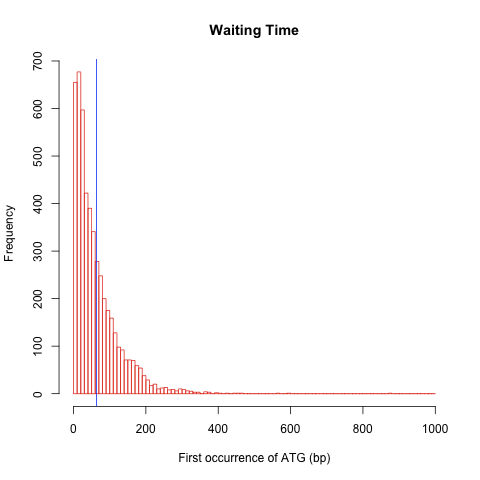
\includegraphics[scale=.75]{waiting-time-atg.png}
\end{center}

%%%%%%%%%%%%%%%%%%%%%%%%%%%%%%%%%%%%%%%%%%%%%%%%%%
\problem

First, let us consider the sequence $YRYR$. Let $\mu_n$ be the probability that we observe $YRYR$ ending at position $n$, $\mu$ be the expected waiting time, and $p$ and $q$ be the probabilities of observing $Y$ and $R$, respectively. We can model the expected waiting time as follows.
\begin{eqnarray}
  p^{2}q^{2} &=& \mu_{n} + \mu_{n - 2}pq \nonumber \\
             &=& \frac{1}{\mu} + \frac{1}{mu}pq \nonumber \\
             &=& \frac{1}{\mu}(1 + pq) \nonumber \\
             &=& \frac{1 + pq}{p^{2}q^{2}}
\end{eqnarray}
If $p = q = 0.5$, then the expected waiting time is 20.

Now consider the sequence $RYRR$. Again, let $\mu_n$ be the probability that we observe $RYRR$ ending at position $n$, $\mu$ be the expected waiting time, and $p$ and $q$ be the probabilities of observing $Y$ and $R$, respectively. We can model the expected waiting time as follows.
\begin{eqnarray}
  p^{2}q^{2} &=& \mu_{n} + \mu_{n - 3}p^{2}q \nonumber \\
             &=& \frac{1}{\mu} + \frac{1}{mu}p^{2}q \nonumber \\
             &=& \frac{1}{\mu}(1 + p^{2}q) \nonumber \\
             &=& \frac{1 + p^{2}q}{p^{3}q}
\end{eqnarray}
If $p = q = 0.5$, then the expected waiting time is 18.

To verify these values empirically, I converted my 5000 random sequences from the alphabet $\{A, C, G, T\}$ to $\{ R, Y\}$ so that the expected composition of each sequence was $P_R = 0.5, P_Y = 0.5$. I then determined the position of the first occurrence of $YRYR$ and $RYRR$ in each sequence. The observed means were 20.25 and 17.80 (respectively), the observed variances were 281.64 and 206.70 (respectively), and the distributions of waiting times (with means highlighted in blue) are shown below.

\begin{center}
  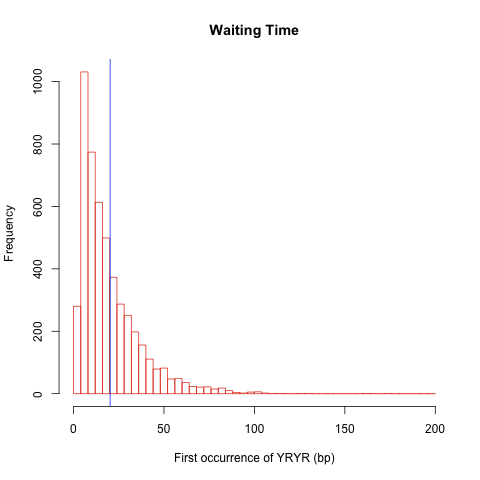
\includegraphics[scale=.4]{waiting-time-yryr.png}
  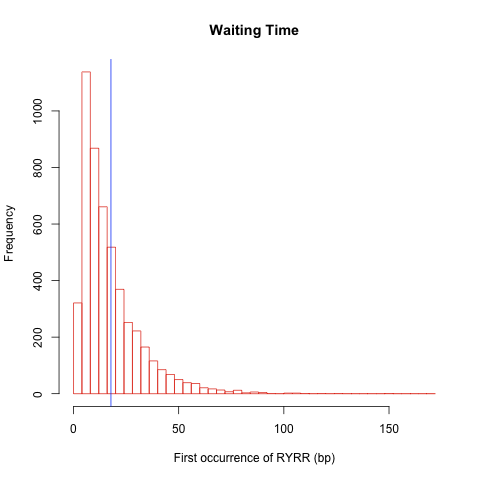
\includegraphics[scale=.4]{waiting-time-ryrr.png}
\end{center}

\end{document}
